\documentclass[aspectratio=169,xcolor=pdftex,dvipsnames,table]{beamer}\usepackage[]{graphicx}\usepackage[]{xcolor}
% maxwidth is the original width if it is less than linewidth
% otherwise use linewidth (to make sure the graphics do not exceed the margin)
\makeatletter
\def\maxwidth{ %
  \ifdim\Gin@nat@width>\linewidth
    \linewidth
  \else
    \Gin@nat@width
  \fi
}
\makeatother

\definecolor{fgcolor}{rgb}{0.345, 0.345, 0.345}
\newcommand{\hlnum}[1]{\textcolor[rgb]{0.686,0.059,0.569}{#1}}%
\newcommand{\hlstr}[1]{\textcolor[rgb]{0.192,0.494,0.8}{#1}}%
\newcommand{\hlcom}[1]{\textcolor[rgb]{0.678,0.584,0.686}{\textit{#1}}}%
\newcommand{\hlopt}[1]{\textcolor[rgb]{0,0,0}{#1}}%
\newcommand{\hlstd}[1]{\textcolor[rgb]{0.345,0.345,0.345}{#1}}%
\newcommand{\hlkwa}[1]{\textcolor[rgb]{0.161,0.373,0.58}{\textbf{#1}}}%
\newcommand{\hlkwb}[1]{\textcolor[rgb]{0.69,0.353,0.396}{#1}}%
\newcommand{\hlkwc}[1]{\textcolor[rgb]{0.333,0.667,0.333}{#1}}%
\newcommand{\hlkwd}[1]{\textcolor[rgb]{0.737,0.353,0.396}{\textbf{#1}}}%
\let\hlipl\hlkwb

\usepackage{framed}
\makeatletter
\newenvironment{kframe}{%
 \def\at@end@of@kframe{}%
 \ifinner\ifhmode%
  \def\at@end@of@kframe{\end{minipage}}%
  \begin{minipage}{\columnwidth}%
 \fi\fi%
 \def\FrameCommand##1{\hskip\@totalleftmargin \hskip-\fboxsep
 \colorbox{shadecolor}{##1}\hskip-\fboxsep
     % There is no \\@totalrightmargin, so:
     \hskip-\linewidth \hskip-\@totalleftmargin \hskip\columnwidth}%
 \MakeFramed {\advance\hsize-\width
   \@totalleftmargin\z@ \linewidth\hsize
   \@setminipage}}%
 {\par\unskip\endMakeFramed%
 \at@end@of@kframe}
\makeatother

\definecolor{shadecolor}{rgb}{.97, .97, .97}
\definecolor{messagecolor}{rgb}{0, 0, 0}
\definecolor{warningcolor}{rgb}{1, 0, 1}
\definecolor{errorcolor}{rgb}{1, 0, 0}
\newenvironment{knitrout}{}{} % an empty environment to be redefined in TeX

\usepackage{alltt}
% \documentclass[notes,aspectratio=169,xcolor=pdftex,dvipsnames,table]{beamer}

%\setbeameroption{show notes}

\usepackage{bm,graphicx,amsmath,tikz} %fancybox,
\usepackage{color}%,textpos}
\usepackage[round]{natbib}
\usepackage[normalem]{ulem}
\usepackage{hyperref}
\usepackage{lastpage}
\usepackage{array}
\usepackage{color}
\usepackage{framed}

% Define Western colours
\definecolor{western}{rgb}{.306,.152,.524}
\definecolor{westerngray}{rgb}{.512,.508,.524}

%% Define BEAMER colours
\setbeamercolor{frametitle}{bg=western,fg=white}
\setbeamercolor{framesubtitle}{bg=western,fg=black}
\setbeamercolor{title}{fg=white,bg=western}
\setbeamercolor{author}{fg=white,bg=western}
\setbeamercolor{institute}{fg=white,bg=western}
\setbeamercolor{date}{fg=white,bg=western}

%% Set BEAMER fonts
\setbeamerfont{title}{shape=\bf}
\setbeamerfont{frametitle}{shape=\sc,size=\Large}
\setbeamerfont{framesubtitle}{shape=\sc,size=\Large}
\setbeamerfont{footline}{shape=\sc}

%% Define BEAMER toc
\setbeamercolor{section in toc}{fg=western}
\setbeamercolor{subsection in toc}{fg=westerngray}
\setbeamertemplate{sections/subsections in toc}[ball]

%% Define BEAMER background
\setbeamercolor{background canvas}{bg=white}

%% Define BEAMER footer
\setbeamertemplate{navigation symbols}{}
\setbeamercolor{footline}{fg=white,bg=western}
\setbeamertemplate{footline}{%
  \begin{beamercolorbox}[wd=\paperwidth]{footline}
    \vskip5pt

    \hspace{.1in}
    \raisebox{.05in}{
      \scriptsize{\bf \insertshorttitle }
    }
    \hfill
    \raisebox{.05in}{
      \scriptsize{\bf \insertframenumber/\pageref{LastPage}}
    }
    \hspace{5pt}

    \vskip5pt
  \end{beamercolorbox}
}

%% Define BLOCK environment
\setbeamercolor{block title}{fg=western}
\setbeamerfont{block title}{series=\bfseries}

%% Define ENUMERATE and ITEMIZE environements
\setbeamertemplate{itemize item}[ball]
\setbeamertemplate{enumerate item}[ball]
\setbeamercolor{item projected}{bg=western}

%% Define BEAMER toc
\setbeamercolor{sections/subsections in toc}{fg=blue!75}
\setbeamertemplate{sections/subsections in toc}[ball]

%% Define SECTION openings
\AtBeginSection[]{
}

\title[SS2857 -- Lecture 6]{SS2857 Probability and Statistics 1\\
  Fall 2024\\
  \vspace{.2in}
  Lecture 6}

\date{Revised 30/09/24}



\IfFileExists{upquote.sty}{\usepackage{upquote}}{}
\begin{document}

{
\setbeamertemplate{footline}{}
\setbeamercolor{background canvas}{bg=western}

\begin{frame}
  \maketitle
\end{frame}
}


\begin{frame}{Chapter 2 Summary Exercise}
  \begin{block}{Activity}
  
  Please take two tickets from the desk at the front of the room. You may choose:
  \begin{itemize}
  \item Two Brown
  \item Two Blue
  \item One Brown and one Blue
  \end{itemize}
  \end{block}
\end{frame}

\begin{frame}{Chapter 2 Summary Exercise}
  \begin{block}{Activity}
  
  
  \begin{itemize}
  \item Move about the room.
  \item  When I say "stop" trade one ticket with someone close to you.
  \item You should end up with one old ticket and one new ticket.
  \item Return to your seat.
  \end{itemize}
  \end{block}
\end{frame}

\begin{frame}
  \begin{center}
    \Large{\textbf{Chapter 2 Summary Exercise}}
    
    \Large{Hardy-Weinberg Equilibrium}

    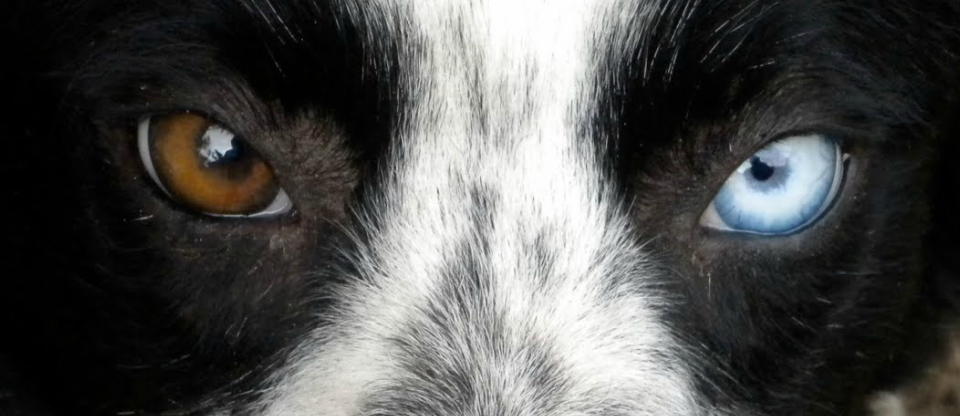
\includegraphics[height = .6\textheight]{1412513462}
  \end{center}
\end{frame}

\begin{frame}{Chapter 2 Summary Exercise}
 
  \begin{block}{Background: Genotypes and Phenotypes}
  \begin{center}
  \url{https://www.youtube.com/watch?v=ZmE0Q4no5Pk}
  \end{center}
  \end{block}
\end{frame}

\begin{frame}{Chapter 2 Summary Exercise}
  
  \begin{block}{Background: Eye Colour}
  \begin{center}
    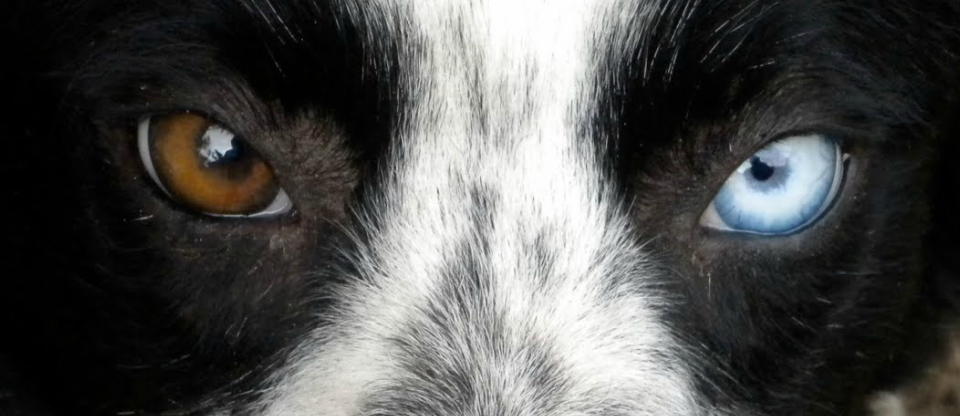
\includegraphics[height = .3\textheight]{1412513462}
  \end{center}
  
  \medskip
  Alleles:
  \begin{itemize}
  \item $A$ -- brown eyes (dominant)
  \item $a$ -- blue eyes (recessive)
  \end{itemize}
  \end{block}
\end{frame}

\begin{frame}{Chapter 2 Summary Exercise}

  \begin{block}{Background: Eye Colour}
  Your genotype is determined by the pair of alleles you have and your phenotype is your eye-colour. 
  
  \begin{center}
  \begin{tabular}{c|cc}
  & \multicolumn{2}{c}{Phenotype}\\
  Genotype & Brown & Blue\\
  \hline
  \hline
  AA & X & \\
  Aa & X & \\
  aa &   & X\\
  \end{tabular}
  \end{center}

  \end{block}
\end{frame}

% The scenario presented in the video assumes that the parents' genotypes are known. In that case, it's easy
% to predict the probabilities associated with the possible offspring.
% We are going to consider what happens when the parents genotypes are not known and instead selected from a
% population.

\begin{frame}{Chapter 2 Summary Exercise}
  \begin{block}{Question 1}
   Suppose that a population contains only homozygotes: 
   \begin{itemize}
   \item $n_{AA}$ is the numbers of people with genotype $AA$, and 
   \item $n_{aa}$ is the numbers of people with genotype $aa$. 
   \end{itemize}
   
   The total population size is
   $$
   n=n_{AA}+n_{aa}.
   $$
   
  \medskip
  
  Suppose that an offspring is formed from two randomly selected parents. What is the probability that the offspring has each of the genotypes?
  \end{block}

\end{frame}

\begin{frame}
  \begin{block}{Question 2}
  Suppose that the population is large so that $n_{AA}$, $n_{Aa}$, and $n_{aa}$ are all much bigger than 1. 
  
  \medskip
  Show that
  $$
  P(G_{AA}) \approx p^2, \quad P(G_{Aa)}=2p(1-p), \quad P(G_{aa)}=\textcolor{red}{(1-p)^2}
  $$
  where $p$ is the proportion of the allele $A$ in the parent population.
  \end{block}
\end{frame}

\begin{frame}{Chapter 2 Summary Exercise}
  \begin{block}{Question 3}
     Suppose now that the population contains all three genotypes:
     \begin{itemize}
    \item $n_{AA}$ is the numbers of people with genotype $AA$,
    \item $n_{Aa}$ is the numbers of people with genotype $Aa$, and
    \item $n_{aa}$ is the numbers of people with genotype $aa$. 
     \end{itemize}
   
   The total population size is
   $$
   n=n_{AA}+n_{Aa}+n_{aa}.
   $$
   
   \medskip
   
    Suppose that an offspring is formed from two randomly selected parents. Show that the same result occurs.
  \end{block}
\end{frame}

\begin{frame}{Chapter 2 Summary Exercise}

  \begin{block}{Hardy-Weinberg Equilibrium}
  A population is said to undergo random mating if:
  
  \begin{enumerate}[1)]
  \item the two alleles an offspring inherits from each parent are independent, and
  \item the probability that each allele takes a specific form is equal to the proportion of that allele in the parent population.
  \end{enumerate}
  \end{block}
  
  \medskip
  
  In this case, the genotype frequencies of a gene with one dominant and one recessive allele will remain close to $p$, $2p(1-p)$, and $(1-p)^2$ where $p$ is the frequence of the dominant allele.
\end{frame}

\begin{frame}{Chapter 2 Summary Exercise}

\begin{block}{Question 4}
Suppose that a population in Hardy-Weinberg equilibrium contains $n_B$ people with brown eyes and $n_b=n-n_B$ people with blues. 

\medskip

What is the probability that a randomly selected person has each of the possible genotypes?
\end{block}
\end{frame}

\begin{frame}{Chapter 2 Summary Exercise}

\begin{block}{Question 5}
Suppose that a population in Hardy-Weinberg equilibrium contains $n_B$ people with brown eyes and $n_b=n-n_B$ people with blues. 

\medskip

What is the probability that a randomly selected person has each of the possible genotypes given that they have brown eyes?
\end{block}
\end{frame}

\begin{frame}{Chapter 2 Summary Exercise}

\begin{block}{Question 6}
Suppose that a population in Hardy-Weinberg equilibrium contains $n_B$ people with brown eyes and $n_b=n-n_B$ people with blues. 

\medskip

What is the probability that a randomly selected person has each of the possible genotypes given that they have brown eyes?
\end{block}
\end{frame}

\begin{frame}
  \begin{center}
    \Large{\textbf{Questions?}}
  \end{center}
\end{frame}


\end{document}
